% Define o tipo de documento
\documentclass[landscape]{slides}

% Importa os caracteres latinos
\usepackage[latin1]{inputenc}
\usepackage[T1]{fontenc}

% Importa os pacotes para inclusao de graficos, links e v�deos
\usepackage{graphicx}
\usepackage{epsfig,color}
\usepackage{hyperref}
\usepackage{multimedia}

% Define o autor
\author{Marcos Marado -- \tt{marcos.marado@ansol.org}}

% Define o titulo
\title{Software Livre em Portugal}

% Define a data
\date{Software Freedom Day 2017 -- Drupal Day Aveiro}

% Da inicio ao documento
\begin{document}

% TITLE

\begin{slide}
\maketitle
\end{slide}

% Sobre a ANSOL
\begin{slide}
ANSOL -- Associa��o Nacional para o Software Livre

Direc��o 2016-2018:
  \begin{itemize}
    \item{} Marcos Marado -- Presidente
    \item{} R�ben Leote -- Vice-Presidente
    \item{} Rui Guimar�es -- Tesoureiro
  \end{itemize}
\end{slide}

% TODO - ter um .tex para cada um destes cap�tulos (Software Livre, ANSOL, SFD,
%   etc.), para que depois possam ser inclu�dos independentemente nas v�rias
%   Apresenta��es

\begin{slide}
O Movimento do Software Livre
\begin{itemize}
\item{} Criado em 1983, por Richard Stallman
\item{} Free Software Foundation fundada em 1985
\item{} Free Software Foundation Europe fundada em 2001
\end{itemize}
\end{slide}

% A ANSOL

% \begin{slide}
% \center{\Huge{ANSOL\\Associa��o Nacional para o Software Livre}}
% \end{slide}

\begin{slide}
ANSOL -- Associa��o Nacional para o Software Livre
\begin{center}
\includegraphics{pct2001-miguelg.jpg}
\end{center}
  \emph{Lan�amento oficial em Outubro de 2001, durante o Porto Cidade Tecnol�gica}

\begin{itemize}
\item{} Associa��o portuguesa sem fins lucrativos 
\item{} divulga��o, promo��o, desenvolvimento, investiga��o e estudo da Inform�tica Livre\ldots
\item{} \ldots e das suas repercuss�es sociais, pol�ticas, filos�ficas, culturais, t�cnicas e cient�ficas
\item{} Sediada na Casa das Associa��es no Porto, mas de �mbito nacional
% \item{} conta com cerca de 80 s�cios
% \item{} quota anual 30 euros (12 euros no caso de estudantes, desempregados e reformados)
\end{itemize}
\end{slide}

% Software Livre

% \begin{slide}
% \center{\Huge{O Software Livre}}
% \end{slide}

% \begin{slide}
% \emph{Software}
% 
% \begin{quote}
% \emph{software} | s. m.
% 
% \emph{software} |softu�re|\\
% (palavra inglesa, de soft, mole + ware, mercadoria)\\
% \emph{substantivo masculino}
% 
% $[$Inform�tica$]$  Conjunto de programas, processos, regras e, eventualmente,
% documenta��o, relativos ao funcionamento de um conjunto de tratamento de
% informa��o (por oposi��o a hardware).
% 
% Plural: softwares.
% \end{quote}
% \hfill \emph{in} \url{https://www.priberam.pt/DLPO/software}
% \end{slide}
% 
% \begin{slide}
% \emph{Software} -- defini��o legal
% 
% \begin{itemize}
% \item{} Lei do Cibercrime refere a exist�ncia de ``programas'', mas n�o produz uma defini��o
% \item{} Lei da Criminalidade Inform�tica (revogada pelo Lei do Cibercrime) definia:
% \begin{quote}
% Programas de computador -- ``Conjunto de instru��es capazes, quando inseridas
% num suporte explor�vel em m�quina, de permitir � m�quina, que tem por fun��es o
% tratamento de informa��es indicar, executar ou produzir determinada fun��o,
% tarefa ou resultado''
% \end{quote}
% \item{} Lei da Criminalidade Inform�tica explicitava ainda a exist�ncia de
%     ``C�digo objecto'' (0s e 1s) e ``C�digo fonte'', ambos considerados programas
%     de computador
% \item{} programas de computador exclu�dos do cat�logo das inven��es protegidas
%     nos termos da Conven��o de Munique sobre a Patente Europeia de 1973
% \item{} Programas de computador considerados como ``obra protegida'' no C�digo
%     do Direito de Autor e dos Direitos Conexos
% \end{itemize}
% 
% \end{slide}

\begin{slide}
Free Software -- Software Livre

\begin{itemize}
\item{} \emph{Free} como \emph{Livre}, n�o gr�tis
\item{} \emph{Livre}, de Liberdade\ldots
\end{itemize}

Que liberdades?
\end{slide}


\begin{slide}
O Software Livre

\begin{small}
No inicio dos anos 80, \emph{Richard M. Stallman} foi o primeiro a formalizar uma maneira de pensar no software sobre a forma de quatro liberdades:
\begin{itemize}
    \item{1� liberdade:} A liberdade de executar o software, para qualquer uso
    \item{2� liberdade:} A liberdade de estudar o funcionamento de um programa e de adapt�-lo �s suas necessidades
    \item{3� liberdade:} A liberdade de redistribuir c�pias
    \item{4� liberdade:} A liberdade de melhorar o programa e de tornar as modifica��es p�blicas de modo que a comunidade inteira beneficie da melhoria
\end{itemize}
O software que siga esses quatro princ�pios � chamado ``Software Livre'' (ou \emph{Free Software}).
\end{small}
\end{slide}

\begin{slide}
\begin{small}
\begin{center}
\input{category.latex} \\
\hfill -- \emph{in} \url{http://www.gnu.org/philosophy/categories.pt-br.html}, CC-SA
\end{center}
\end{small}
\end{slide}

% EXEMPLOS DE SW LIVRE
\begin{slide}
\begin{small}
\begin{itemize}
\item{} Sistema Operativo GNU/Linux
\item{} Android Operating System Project
\item{} OpenOffice -- LibreOffice
\item{} Firefox
\item{} Wordpress
\item{} Servidor Web Apache
\item{} Blender
\item{} Moodle
\item{} \emph{muitos outros...}
\end{itemize}
\end{small}
\end{slide}


\begin{slide}
Licen�as de Software
\begin{small}
\begin{itemize}
  \item{} Licen�as Copyleft -- programas derivados n�o podem acrescentar restri��es � licen�a
  \begin{itemize} 
    \item{} GPL (GNU General Public License)
    \item{} Mozilla Public License (MPL)
    \item{} Microsoft Reciprocal License (Ms-RL)
  \end{itemize}
  \item{} N�o Copyleft
  \begin{itemize} 
    \item{} Modified BSD License
    \item{} Expat License (MIT)
    \item{} Apache License
  \end{itemize}
\end{itemize}
\end{small}
\end{slide}



\begin{slide}
Actividades da Associa��o

\begin{itemize}
\item{} Interven��es no meio pol�tico e legilativo
\begin{itemize}
  \item{} Interver��es e elabora��o de pareceres junto da Comiss�o de Assuntos Constitucionais, Direitos, Liberdades e Garantias do Parlamento Portugu�s
  \item{} Coordena��o com a \emph{Free Software Foundation Europe} para trabalhos em �mbito Europeu, incluindo presen�a no Parlamento Europeu
  \item{} Envolvimento na transposi��o da Directiva Europeia \\InfoSoc para a Legisla��o Portuguesa
%    \begin{itemize}
%        \item{} Directiva Europeia que implementa, pela primeira vez, restri��es de acesso no Direito de Autor
%        \item{} Criminaliza neutraliza��o de DRM
%        \item{} Criminaliza qualquer discuss�o que possa facilitar essa neutraliza��o
%        \item{} Interfere no desenvolvimento de Software Livre
%        \item{} Contributo inicial enviado em 2002, acompanhamento da proposta at� � sua aprova��o em 2004
%        \item{} Mais info: \url{https://ansol.org/politica/eucd}
%    \end{itemize}
  \item{} Campanha contra Patentes de Software, que culminou na sua rejei��o pelo Parlamento Europeu % \includegraphics{patentes.png}
  \item{} Portugal � o primeiro pa�s a ter uma Lei das Normas Abertas                                %
  \item{} Participa��o na campanha internacional contra o ACTA                                       % \includegraphics{ACTA.png}
  \item{} Combate � Lei da C�pia Privada
  \item{} Portugal na linha da frente na defesa dos consumidores contra o DRM
\end{itemize}
\end{itemize}
\end{slide}

\begin{slide}
\begin{itemize}
\item{} Lan�amento do Portal ``Transpar�ncia na AP'' em 2009
\\ \includegraphics{transparencia.png}
\item{} Sun e ANSOL juntam-se na elabora��o do CD ``Software Livre na Escola'', distribu�do nas escolas pelo Minist�rio da Educa��o
        \\ \includegraphics{CD.png}
\item{} Organiza��o de eventos
\begin{itemize}
  \item{} Porto 2002, Cidade Tecnol�gica - Sistemas Livres % \includegraphics{porto2002.png}
  \item{} Richard Stallman em Portugal                     % \includegraphics{stallman-2003.png}
  \item{} Software Freedom Day     %
  \item{} Document Freedom Day     % \includegraphics{DFD.png}
  \item{} Eu $<3$ Software Livre
\end{itemize}
\end{itemize}
 
    % \item{} OOXML publicado como norma ECMA em 2006, distin��o entre ``norma'' e ``normas abertas''
    %     \\ \includegraphics{OOXML.png}
    % \item{} ANSOL recebe pr�mio ``Software'' dos Pr�mios Exame Inform�tica 2006, em nome da Mozilla Foundation
%\end{itemize}
%\end{slide}
%\begin{slide}
%\begin{itemize}
%    \item{} Campanha para o uso de Software Livre na Administra��o P�blica em 2010, poupan�a estimada em 121 milh�es
%        \\ \includegraphics{AP.png}
%\end{itemize}
%\end{slide}
%\begin{slide}
%    \begin{itemize}
%    \item{} Em 2013 a ANSOL junta-se a outras entidades no apelo � AR para a correc��o da legisla��o relativa ao DRM
%        \\ \includegraphics{DRM.png}
%    \item{} Lei da C�pia Privada volta � agenda Pol�tica Portuguesa em 2014, ANSOL organiza peti��o
%        \\ \includegraphics{PL118.png}
%\end{itemize}
%\end{slide}
%\begin{slide}
%A ANSOL em 2015:
%\begin{itemize}
% \item{} Celebra��o do ``Eu $<3$ Software Livre 2015''
% \item{} Esclarecimento sobre o WMV n�o ser uma norma aberta
% \item{} Celebra��o do Education Freedom Day 2015, em Lisboa
% \item{} Apelo � participa��o no Dia de Ac��o Global contra os Tratados Transatl�nticos
% \item{} Dar a conhecer a Liberdade que vem do Software Livre, no Dia da Liberdade
% \item{} Contesta��o contra os tratados TTIP e CETA nas manifesta��es do $1^o$ de Maio
% \item{} Press Release sobre a aprova��o da Lei da C�pia Privada
% \item{} co-organiza��o do evento ``Workshop de Direitos de Autor e DRM''
% \item{} Assembleia Geral Eleitoral
% \item{} Plano de regulariza��o da situa��o dos s�cios com quotas em atraso
% \item{} Regulariza��o da situa��o dos certificados https dos v�rios sites da ANSOL
% \item{} Forma��o do novo Grupo de Trabalho sobre Normas Abertas
% \item{} Forma��o do novo Grupo de Trabalho de WebMasters
% \item{} Apoio na organiza��o do Software Freedom Day 2015, no Porto
% \item{} Regulariza��o da situa��o de associados da EDRi
% \item{} Press release sobre o t�rmino da campanha sobre leitores de PDF da FSFE
% \item{} Assembleia Geral, para altera��o dos estatutos e regulamento interno
% \item{} Escritura��o nos novos estatutos da ANSOL
% \item{} Assinatura de protocolo com a Casa das Associa��es, formalizando a sedia��o da ANSOL naquele espa�o
% \item{} Participa��o no semin�rio ``O Regulamento Nacional de Interoperabilidade Digital e a ado��o de Normas Abertas pela Administra��o P�blica''
% \item{} Participa��o na consulta p�blica sobre normas abertas
% \item{} Manuten��o da lista de incumprimentos do RNID
%\end{itemize}
%
%A ANSOL em 2016\ldots depende de todos!
\end{slide}

% \begin{slide}
% \includegraphics{eventos.png}
% \end{slide}
% 
% % O SFD
% 
% \begin{slide}
% \center{\Huge{O Software Freedom Day}}
% \end{slide}
% 
% \begin{slide}
% O Software Freedom Day
% \begin{center}
% \includegraphics{sfd-2015.png}
% \end{center}
% \emph{Mapa de Eventos SFD 2015 registados a 17 de Agosto} % TODO - actualizar
% 
% \include{sfd-teams}
% 
% \emph{Vis�o:} Potenciar todos a ligar, criar e partilhar livremente num mundo digital participat�rio, transparente e sustent�vel.
% 
% Objectivos
% \begin{itemize}
% \item{} Celebrar o Software Livre e as pessoas por detr�s dele
% \item{} Promover o conhecimento geral sobre Software Livre, e encorajar a adop��o de Software Livre e Normas Abertas
% \item{} Criar igualidade de acesso a oportunidades atrav�s do uso de tecnologias participat�rias
% \end{itemize}
% \end{slide}
% 
% \begin{slide}
% O Software Freedom Day -- Objectivos \emph{(continua��o)}
% \begin{itemize}
% \item{} Promover um di�logo construtivo sobre as responsabilidades e os direitos na Sociedade de Informa��o
% \item{} Ser inclusivo de organiza��es e indiv�duos que partilham a nossa Vis�o
% \item{} Ser pragm�tico, transparente e respons�vel enquanto organiza��o
% \end{itemize}
% \end{slide}
% 
% % Normas Abertas
% \begin{slide}
% \center{\Huge{Normas Abertas}}
% \end{slide}
% 
% \input{rnid.tex}
% 
% % Teoria e pr�tica de m�os dadas - o exemplo do leftpad
% \begin{slide}
%     Filosofia e c�digo -- duas faces da mesma moeda
%     \begin{verbatim}
% // "license": "WTFPL"
% module.exports = leftpad;
% function leftpad (str, len, ch) {
%   str = String(str);
%   var i = -1;
%   if (!ch && ch !== 0) ch = ' ';
%   len = len - str.length;
%   while (++i < len) {
%     str = ch + str;
%   }
%   return str;
% }
%     \end{verbatim}
% \begin{tiny}\url{http://qz.com/646467/how-one-programmer-broke-the-internet-by-deleting-a-tiny-piece-of-code/}\end{tiny}
% \end{slide}
% 
% \begin{slide}
% \begin{itemize}
% \item{} trademark
% \item{} patentes de software
% \item{} npm takedown
% \item{} remo��o de todos os m�dulos
% \item{} npm?
% \item{} WTFPL (vs. Apache 2.0, que protege os utilizadores de eventuais patentes de software)
% \end{itemize}
% \end{slide}

%% VANTAGENS 
% FIXME: De futuro, quereremos ter a nossa pr�pria lista de vantagens, de acordo com os nossos crit�rios. Algumas notas que ficaram da �ltima reuni�o sobre o tema:
% * poss�vel modifica��o permitiu muita gente a modificar e a distribuir modifica��es o que melhorou muito o software muito mais rapidamente do que se nao fosse SL
% * Migra��o da Tranquilidade?
% At� l�, a lista de vantagens aqui apresentadas � inspirada em http://open-source.gbdirect.co.uk/migration/benefit.html
\begin{slide}
As vantagens do Software Livre
  \begin{itemize}
    \item{} Flexibilidade e Liberdade
    \item{} Confiabilidade
    \item{} Estabilidade
    \item{} Auditabilidade
    \item{} Suporte e Responsabilidade
    \item{} Custo
  \end{itemize}
\end{slide}
\begin{slide}
As vantagens do Software Livre -- Flexibilidade e Liberdade
  \begin{itemize}
    \item{} Flexibilidade -- a capacidade de escolher solu��es adequadas para as necessidades dos utilizadores
    \item{} Se os requisitos de neg�cio mudam, as solu��es n�o devem estar constrangidas pelo software
    \item{} O uso de normas abertas para a interoperabilidade
    \item{} as melhores solu��es podem ser seleccionadas para componentes particulares na arquitectura
    \item{} se as solu��es t�m boa interoperabilidade, o neg�cio pode evitar o lock-in a um fornecedor em particular, evitando depend�cia
    \item{} Os modelos de Software Livre n�o promovem vendor-lock in, pelo que ades�o a normas abertas � tipicamente alta
    \item{} Para casos em que n�o existem normas abertas, auditoria do c�digo fonte impede o uso de formatos propriet�rios como forma de lock-in
    \item{} Competi��o centra-se na qualidade das funcionalidades
    \item{} Liberdade ao n�o ter um fornecedor apenas
    \item{} Liberdade de modificar o seu software
  \end{itemize}
\end{slide}
\begin{slide}
As vantagens do Software Livre -- Confiabilidade
  \begin{itemize}
    \item{} Confiabilidade -- aus�ncia de defeitos que causam opera��o incorrecta
    \item{} falhas de performance; falhas de conformidade com normas; falhas de seguran�a
    \item{} Falhas graves tendem a ser resolvidas num prazo de horas depois de ser descobertas, em muito devido ao acesso ao c�digo fonte
    \item{} \emph{patch} vs. nova vers�o
    \item{} ciclo de vida de um bug diferente entre o software livre e o propriet�rio
    \item{} o impacto dos \emph{early adopters}, tanto em correc��es como em novas vers�es
  \end{itemize}
\end{slide}
\begin{slide}
As vantagens do Software Livre -- Estabilidade
  \begin{itemize}
    \item{} Estabilidade vs. Actualiza��es
    \item{} \emph{vendor push}: Altera��o de formatos, fim de suporte, falta de correc��es ao software
    \item{} Garantia de possibilidade de migra��o de dados
    \item{} Acesso ao c�digo fonte providencia forma de extens�o de tempo de vida do software
    \item{} Escolha quanto � actualiza��o fica a cargo do utilizador, n�o do fornecedor
  \end{itemize}
\end{slide}
\begin{slide}
As vantagens do Software Livre -- Auditabilidade
  \begin{itemize}
    \item{} Seguran�a, aus�ncia de \emph{backdoors}, ades�o �s normas e flexibildade em altera��es futuras: podem ser promessas no software propriet�rio, mas s� garantias com acesso ao c�digo fonte
    \item{} inspec��o pontual e informal vs. auditorias rigorosas
      \begin{itemize}
        \item{} O caso InterBase: \emph{backdoor} com 7 anos descoberta e corrigida meio ano ap�s lan�amento de vers�o software livre
        \item{} A \emph{backdoor} tinha sido introduzida propositadamente por engenheiros da Borland
      \end{itemize}
    \item{} inspec��o e certifica��o por terceiros
    \item{} a fal�cia da \emph{security through obscurity}
  \end{itemize}
\end{slide}
\begin{slide}
As vantagens do Software Livre -- Suporte e Responsabilidade
  \begin{itemize}
    \item{} Contratos de suporte: dos gen�ricos aos personalizados
    \item{} Suporte interno ou externo, � medida (e o ex. da Ada)
      \begin{itemize}
        \item{} Ada � uma linguagem espec�fica para o contexto de sistemas militares, industriais e aeroespaciais que sejam \\
          \emph{mission-critical} e \emph{safety-critical}
        \item{} A ``ACT Europe'' foi fundada em 1996 para providencial suporte comercial a usos industriais e militares do Ada
      \end{itemize}
    \item{} V�rios modelos de neg�cio em torno do Suporte
      \begin{itemize}
        \item{} Zope -- Produ��o de Software Livre; maior parte do lucro vindo de presta��o de servi�os e suporte
        \item{} Servi�os de Consultadoria de Software Livre
      \end{itemize}
    \item{} A verdadeira necessidade de suporte, quando o c�digo � do utilizador
    \item{} O mito da responsabilidade no software propriet�rio \\ (ler EULAs)
  \end{itemize}
\end{slide}
\begin{slide}
As vantagens do Software Livre -- Custo
  \begin{itemize}
    \item{} libre vs. gratis
    \item{} Pre�o vs. TCO
    \item{} Generalidades sobre o TCO de Software Livre
      \begin{itemize}
        \item{} Possibilidade de pre�o zero
        \item{} Possibilidade de n�o necessidade de contabiliza��o de n�mero de c�pias em uso
        \item{} Prov�vel necessidade reduzida de actualiza��es
        \item{} Vulnerabilidade a v�rus quase-zero
        \item{} Suposta menor vulnerabilidade a falhas de seguran�a
        \item{} Suposta possibilidade de prolongamento do tempo de vida com requisitos de hardware baixos
        \item{} Uma melhor ades�o a normas abertas permite a competi��o, reduzindo o lock-in a pre�os monopolistas
        \item{} Disponibiliza��o de c�digo fonte torna o software resiliente a descontinua��o de produtos ou extin��o de fornecedores
        \item{} Estrat�gia financeira ditada pelo utilizador e n�o pelo fornecedor
      \end{itemize}
  \end{itemize}
\end{slide}

%% MODELOS DE NEG�CIO
\begin{slide}
  Modelos de Neg�cio com Software Livre
  \begin{itemize}
    \item Oferecer o software para vender hardware (IBM, ...)
    \item Licenciamento permite inclus�o em programas n�o-livres (MySQL)
    \item Publicar o software sem c�digo, libertando-o ap�s algum tempo
    \item Software base � livre, os extras n�o o s�o
    \item Partilha de custos de desenvolvimento
  \end{itemize}
\end{slide}
\begin{slide}
  Modelos de Neg�cio com Software Livre (cont.)
  \begin{itemize}
    \item Contratos de assist�ncia t�cnica
    \item Desenvovimento de funcionalidades novas
    \item Forma��o
    \item Consultoria e adapta��o do programa
  \end{itemize}
\end{slide}

%% ENVOLVE-TE
\begin{slide}
\center{\Huge{Envolve-te!}}
\end{slide}

\begin{slide}
Save Code Share -- \url{https://savecodeshare.eu/}

\center{\includegraphics{save-code-share.png}}
\end{slide}

\begin{slide}
% link to the site where the video is
\center{\href{https://www.youtube.com/watch?v=iuVUzg6x2yo}{\includegraphics{pmpc-video.png}}}
% embed movie link (doesn't work in many PDF readers)
%\movie[]{\includegraphics{pmpc-video.png}}{pmpc_desktop.mp4}
% embed movie inside the PDF - works in even less PDF readers, so I didn't even bothered with the code for that
\end{slide}

\begin{slide}
  ANSOL-geral -- \url{http://listas.ansol.org/mailman/listinfo/ansol-geral}
  \includegraphics{ansol-geral.png}
\end{slide}

\begin{slide}
  \center{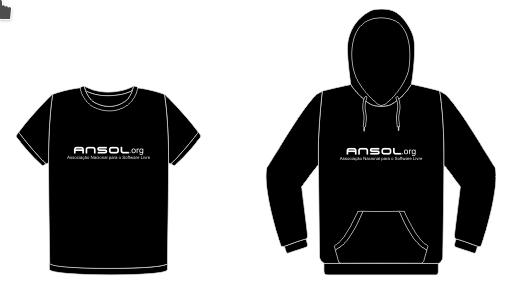
\includegraphics{ANSOL-freewear.png}} \\
  t-shirt: 18\euro\ -- 3\euro\ doados para a ANSOL \\
  sweatshirt: 25\euro\ -- 3\euro\ doados para a ANSOL
\end{slide}

\begin{slide}
  \includegraphics[scale=0.8]{ANSOL-flyers.png}
\end{slide}


% Sobre as Comunidades Portuguesas de Software Livre
%% Conte�do maioritariamente retirado de https://ansol.org/comunidades
\begin{slide}
Comunidades Portuguesas de Software Livre
  \begin{itemize}
    \item{} Associa��es
    \item{} Comunidades
    \item{} Ensino
    \item{} Distribui��es
    \item{} Blogs
  \end{itemize}

  \url{https://ansol.org/comunidades}
\end{slide}

%% QUEST�ES
\begin{slide}
\center{\Huge{QUEST�ES?}}

\emph{http://ansol.org} \\
\emph{http://fsfe.org} \\
\emph{http://fsf.org} \\
\emph{https://github.com/marado/ANSOL-presentation} \\
\emph{http://listas.ansol.org/mailman/listinfo/ansol-geral} \\
\emph{https://savecodeshare.eu} \\
\emph{https://publiccode.eu}
\end{slide}

\end{document}
